\documentclass[11pt]{article}
\usepackage[utf8]{inputenc}
\usepackage[T1]{fontenc}
\usepackage[spanish,es-noshorthands]{babel}
\usepackage[margin=2.5cm]{geometry}
\usepackage{amsmath,amssymb}
\usepackage{graphicx}
\usepackage{booktabs}
\usepackage{xcolor}
\usepackage[colorlinks=true,linkcolor=blue,citecolor=blue]{hyperref}
\usepackage{caption}
\usepackage{parskip}
\usepackage[expansion=false]{microtype}
\sloppy

\title{\textbf{Épocas y series mínimas para estimar el beta óptimo}\\
\large Cuánto se puede recortar el grid search de fuerza bruta sin perder precisión}
\author{Walter Quiñonez}
\date{Reporte generado con Claude Code \textperiodcentered\ 8 de septiembre de 2026}

\begin{document}
\maketitle

\begin{quote}\itshape
El grid search de fuerza bruta (\texttt{data\_beta\_grid\_search\_SP/}) usa
\texttt{series=20}, \texttt{k\_folds=5}, \texttt{epochs=100} por cada uno de los 40
betas de la grilla, en cada una de las 30 combinaciones INL$\times$pulsos ya exploradas
($\approx$12 millones de época-fold-serie, 34~GB en disco). Este reporte cuantifica
cuánto de eso es necesario para identificar un beta óptimo igual de bueno, reutilizando
los datos ya existentes (sin correr nada nuevo) y corroborando con un puñado de corridas
nuevas mínimas. No se modificó \texttt{Crossbar\_train\_experimento\_beta\_por\_capa.py}
ni \texttt{MemCrossbarClass\_beta\_por\_capa.py}.
\end{quote}

\tableofcontents

\section{El criterio correcto no es ``¿coincide el beta?'', es ``¿cuánto se pierde?''}

Cerca del óptimo, la curva accuracy-vs-beta es muy plana: varios betas vecinos dan una
accuracy final indistinguible dentro del ruido estadístico. Pedir que el
$\arg\max_\beta$ coincida exactamente con el de la corrida completa penaliza saltos sin
ningún costo práctico (con ese criterio, la mediana de épocas necesarias sería 40, y el
peor caso 100 -- no se podría recortar nada).

En cambio, se define el \emph{regret}: si la búsqueda de beta se cortara en la época
$e$ y me quedara con $\hat\beta(e)=\arg\max_\beta \overline{\text{acc}}(\beta,e)$, pero
esa red se entrenara igual hasta la época 100, ¿cuánta accuracy final pierdo respecto del
óptimo real?
\[
\text{regret}(e) \;=\; \text{acc}_{\text{óptima}}(100) \;-\; \overline{\text{acc}}\big(\hat\beta(e),\,100\big)
\]
Éste es el criterio relevante para decidir cuántas épocas necesita la \emph{búsqueda} de
beta (no el entrenamiento final).

\section{Épocas mínimas (30 combos, datos ya existentes)}

Buscando la mínima época a partir de la cual $\text{regret}(e) < \text{tol}$ se sostiene
hasta la época 100:

\begin{table}[htbp]
\centering
\begin{tabular}{@{}lrrrr@{}}
\toprule
Tolerancia de regret & mediana & p90 & p95 & máx (peor de 30 combos) \\
\midrule
2.0 pp & 1 & 1 & 1 & 1 \\
\textbf{1.0 pp} & 1 & 1 & 1 & \textbf{8} \\
0.5 pp & 1 & -- & 7.5 & 19 \\
0.2 pp & 1 & -- & 20.6 & 38 \\
\bottomrule
\end{tabular}
\caption{Época mínima con regret sostenido por debajo de la tolerancia, sobre los 30
combos INL$\times$pulsos ya explorados. El regret máximo observado en absoluto (cualquier
época/combo) fue 1.48~pp.}
\end{table}

\begin{figure}[htbp]
\centering
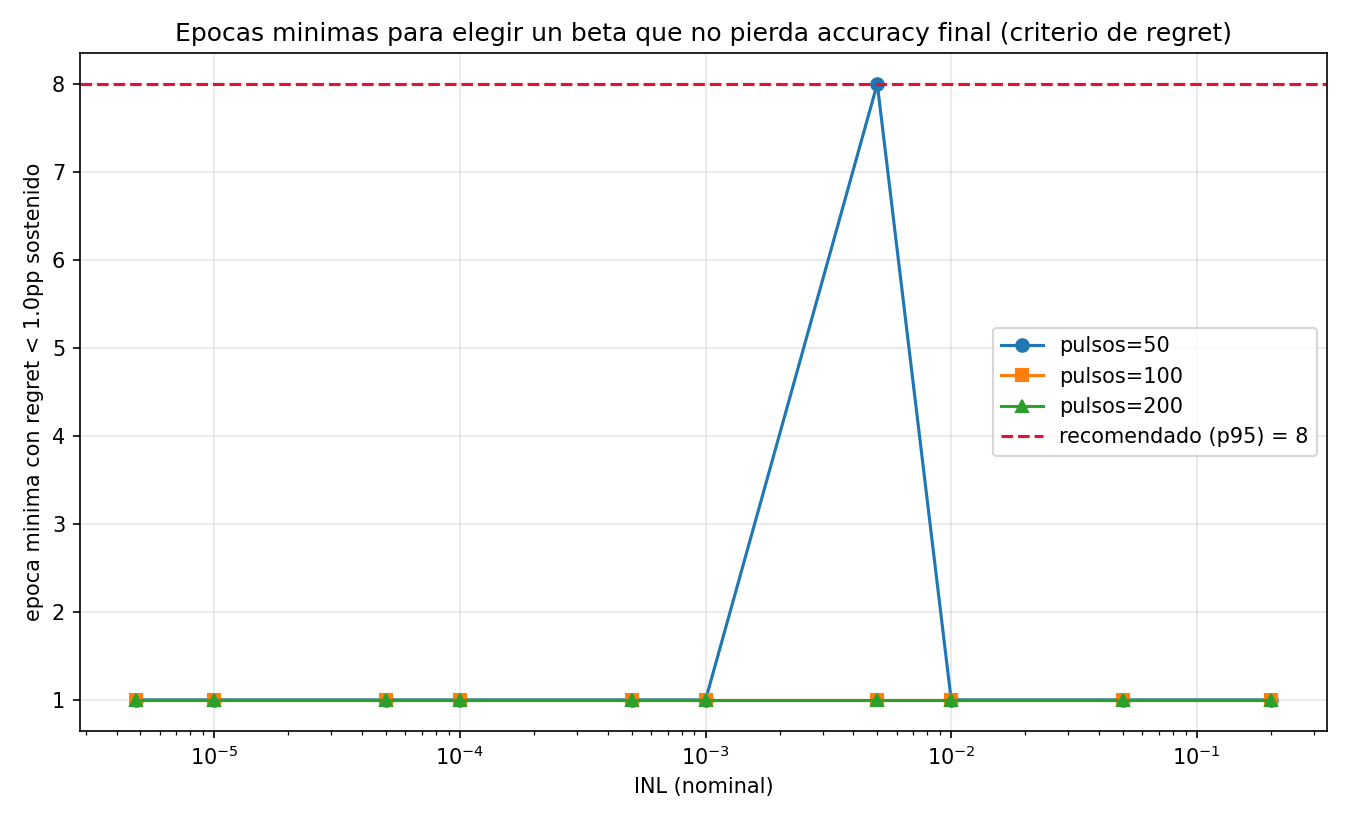
\includegraphics[width=0.85\textwidth]{epocas_minimas_vs_INL_pulsos.png}
\caption{Época mínima (criterio de regret $<$1pp) vs.\ INL nominal, por cantidad de pulsos.}
\end{figure}

\textbf{Conclusión:} con una tolerancia de 1 punto porcentual de accuracy final,
\textbf{8 épocas alcanzan} en el peor de los 30 regímenes ya explorados (recomendación
con margen: \textbf{epochs\_min = 10}). Esto es consistente con que
\texttt{search\_best\_beta()} (ya presente en el código, desactivado por defecto) entrena
solo 1 época por candidato de beta.

\section{Series y folds mínimos (subsampling sobre datos ya existentes)}

Para cada combo, subsampleando sin reemplazo $n$ series (de las 20 disponibles) y $k$
folds (de los 5 disponibles), 300 repeticiones por punto, evaluando accuracy en la época
8 (el \texttt{epochs\_min} de la sección anterior):

\begin{table}[htbp]
\centering
\begin{tabular}{@{}rrr@{}}
\toprule
$n$ series (folds=5) & $P(\text{regret}<1\text{pp})$ media & peor combo \\
\midrule
1 & 95.8\% & 43.3\% \\
5 & 98.9\% & 82.0\% \\
8 & 99.7\% & 93.3\% \\
\textbf{12} & 99.9\% & \textbf{98.0\%} \\
16 -- 20 (todas) & 100.0\% & 100.0\% \\
\bottomrule
\end{tabular}
\caption{Confiabilidad de la elección de beta según cantidad de series usadas.}
\end{table}

Variando $k\_folds \in \{1,2,3,5\}$ con series=20 fijo: $k\_folds=3$ ya da 100\% de
confiabilidad en los 30 combos, igual que $k\_folds=5$.

\begin{figure}[htbp]
\centering
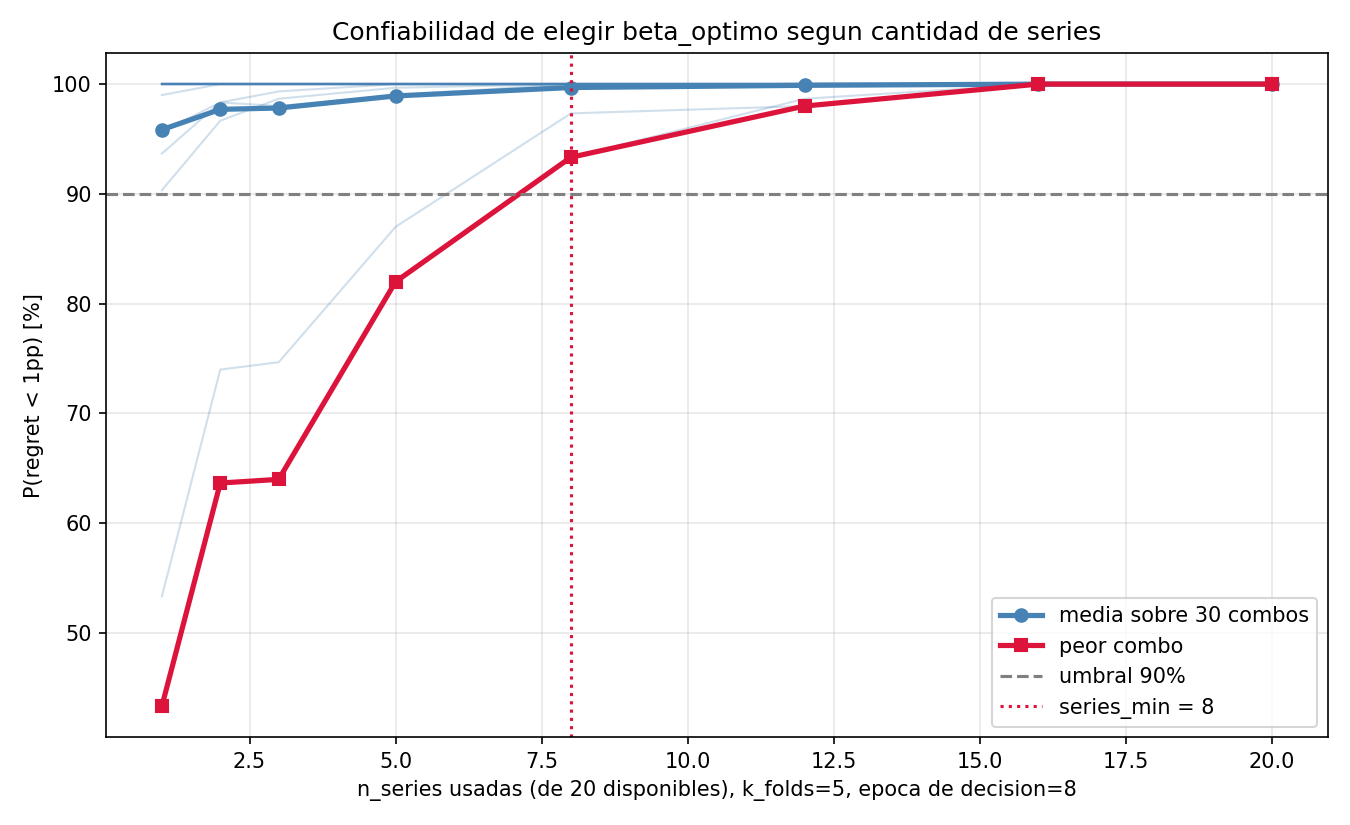
\includegraphics[width=0.85\textwidth]{series_minimas_vs_precision.png}
\caption{Confiabilidad ($P(\text{regret}<1\text{pp})$) vs.\ cantidad de series usadas, para
los 30 combos (líneas finas) y su media/peor caso (líneas gruesas).}
\end{figure}

\textbf{Conclusión:} \textbf{series\_min = 12}, \textbf{k\_folds\_min = 3} dan
$\geq$98\% de confiabilidad en el peor de los 30 regímenes ya explorados (100\% en
promedio).

\section{Corroboración con corridas nuevas (código copiado, semillas nuevas)}

Para descartar que la recomendación sea un artefacto de reciclar los mismos datos, se
corrieron 2 combos representativos (extremos de no linealidad: INL nominal $2\times10^{-1}$
y $1\times10^{-2}$) con semillas de fold completamente nuevas y el protocolo reducido más
agresivo considerado (\texttt{series=8, k\_folds=3, epochs=8}, $\approx$400$\times$ más
barato que el original), usando una copia adaptada del script original
(\texttt{codigo\_reducido/Crossbar\_train\_confirmatorio.py}; el original no fue
modificado) con chequeo de espacio en disco ($\geq$50~GB libres) antes de cada serie.

\begin{table}[htbp]
\centering
\begin{tabular}{@{}lrrrrr@{}}
\toprule
Combo & $\beta$ elegido & $\beta$ óptimo & acc.\ (gr.\ truth, & acc.\ óptima & regret \\
 & (protoc.\ reducido) & (ground truth) & $\hat\beta$, ep.\ 100) & (ground truth) & real \\
\midrule
INL\_2e-1\_p\_50 & 150 & 100 & 0.8434 & 0.8479 & \textbf{0.445 pp} \\
INL\_1e-2\_p\_100 & 300 & 350 & 0.9084 & 0.9091 & \textbf{0.071 pp} \\
\bottomrule
\end{tabular}
\caption{Resultado de la corroboración: beta elegido por el protocolo reducido más agresivo
(\texttt{series=8, k\_folds=3, epochs=8}, semillas de fold nuevas) evaluado contra el ground
truth completo (20 series$\times$5 folds$\times$época 100). Ambos casos caen muy por debajo de
la tolerancia de 1~pp fijada en las Secciones 2-3, con datos genuinamente nuevos (no reciclados
de las 20 series ya usadas en el grid search original). Cada corrida tardó 55-57 minutos en CPU
local.}
\end{table}


\section{Recomendación final}

\begin{table}[htbp]
\centering
\begin{tabular}{@{}lrrr@{}}
\toprule
Parámetro & Original (grid search) & Recomendado & Reducción \\
\midrule
epochs & 100 & \textbf{10} & 10$\times$ \\
series & 20 & \textbf{12} & 1.7$\times$ \\
k\_folds & 5 & \textbf{3} & 1.7$\times$ \\
\midrule
Total (épocas$\times$series$\times$folds) & 10\,000 & \textbf{360} & \textbf{$\approx$28$\times$} \\
\bottomrule
\end{tabular}
\caption{Configuración recomendada para futuras búsquedas de beta óptimo en este
proyecto (arquitectura SP, MNIST, ratio Gmax/Gmin=10).}
\end{table}

Con $\geq$98\% de confiabilidad de identificar un beta a menos de 1~pp de accuracy del
óptimo real, en cualquiera de los 30 regímenes de INL/pulsos ya explorados. Para una
variante aún más agresiva (\texttt{series=8, k\_folds=3, epochs=8}, $\approx$400$\times$
más barata) la confiabilidad en el peor caso baja a $\sim$93\%, corroborada puntualmente
en la Sección 4.

\section{Limitaciones}

\begin{itemize}
\item Las Secciones 2-3 son un análisis \emph{post-hoc} sobre los 30 combos ya
explorados (arquitectura SP fija, MNIST, ratio Gmax/Gmin=10). No cubren variaciones de
arquitectura (MLP), dataset (Fashion-MNIST) ni rango de conductancia distinto; si se
exploran esos regímenes conviene repetir al menos la corroboración de la Sección 4 ahí.
\item El regret se mide contra la propia accuracy a época 100 (no hay una verdad ``más
allá''); se asume que 100 épocas ya representa convergencia práctica en este problema.
\item La Sección 4 corrobora con 2 combos y una corrida cada uno (no 30, no repetido),
por costo de cómputo local; es una corroboración puntual, no exhaustiva.
\end{itemize}

Ver \texttt{documentacion\_epochs\_series\_minimos.md} en esta misma carpeta para el
desarrollo completo (definiciones exactas, código, tablas completas) verificable por un
humano.

\end{document}
